\section{Tebranishlar konturida zaryad, kuchlanish va tok kuchi.}






\begin{enumerate}

\item Ko‘rsatilgan konturlarning qaysi birida so‘nmas elektromagnit tebranishlar hosil bo‘lishi mumkin?

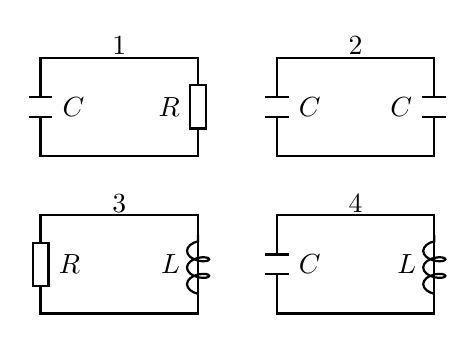
\begin{tikzpicture}[thick, scale=0.5]

    % --- 1-KONTUR (C va R) ---
    \begin{scope}[xshift=0cm, yshift=0cm]
        \draw (0,0) rectangle (4,2.5);
        \node at (2, 2.8) {1};
        % Kondensator C
        \fill[white] (-0.2, 1) rectangle (0.2, 1.5);
        \draw (-0.3, 1) -- (0.3, 1) (-0.3, 1.5) -- (0.3, 1.5);
        \node[right] at (0.3, 1.25) {$C$};
        % Rezistor R
        \draw[fill=white] (3.8, 0.7) rectangle (4.2, 1.8);
        \node[left] at (3.8, 1.25) {$R$};
    \end{scope}

    % --- 2-KONTUR (C va C) ---
    \begin{scope}[xshift=6cm, yshift=0cm]
        \draw (0,0) rectangle (4,2.5);
        \node at (2, 2.8) {2};
        % Kondensator C (chap)
        \fill[white] (-0.2, 1) rectangle (0.2, 1.5);
        \draw (-0.3, 1) -- (0.3, 1) (-0.3, 1.5) -- (0.3, 1.5);
        \node[right] at (0.3, 1.25) {$C$};
        % Kondensator C (o'ng)
        \fill[white] (3.8, 1) rectangle (4.2, 1.5);
        \draw (3.7, 1) -- (4.3, 1) (3.7, 1.5) -- (4.3, 1.5);
        \node[left] at (3.7, 1.25) {$C$};
    \end{scope}

    % --- 3-KONTUR (R va L) ---
    \begin{scope}[xshift=0cm, yshift=-4cm]
        \draw (0,0) rectangle (4,2.5);
        \node at (2, 2.8) {3};
        % Rezistor R
        \draw[fill=white] (-0.2, 0.7) rectangle (0.2, 1.8);
        \node[right] at (0.2, 1.25) {$R$};
        % G'altak L
        \draw[decoration={coil, aspect=0.5, segment length=6pt, amplitude=4pt}, decorate] (4, 0.5) -- (4, 2);
        \node[left] at (3.8, 1.25) {$L$};
    \end{scope}

    % --- 4-KONTUR (C va L - TO'G'RI JAVOB) ---
    \begin{scope}[xshift=6cm, yshift=-4cm]
        \draw (0,0) rectangle (4,2.5);
        \node at (2, 2.8) {4};
        % Kondensator C
        \fill[white] (-0.2, 1) rectangle (0.2, 1.5);
        \draw (-0.3, 1) -- (0.3, 1) (-0.3, 1.5) -- (0.3, 1.5);
        \node[right] at (0.3, 1.25) {$C$};
        % G'altak L
        \draw[decoration={coil, aspect=0.5, segment length=6pt, amplitude=4pt}, decorate] (4, 0.5) -- (4, 2);
        \node[left] at (3.8, 1.25) {$L$};
    \end{scope}

\end{tikzpicture}

\begin{enumerate}[label=\Alph*)]
\item 1.
\item 2.
\item 3.
\item 4.
\item hammasida.
\end{enumerate}

\item Tebranishlar konturidagi zaryadning o‘zgarish qonuni $q=\sin 10t \ (\text{C})$ ko‘rinishiga ega. Tok kuchi tebranishlarining amplituda qiymatini toping (A).
\begin{enumerate}[label=\Alph*)]
\item 0.
\item 0,1.
\item 1.
\item 10.
\item 100.
\end{enumerate}

\item Tebranishlar konturidagi kondensator plastinalaridagi zaryad vaqt o‘tishi bilan $q=10^{-6}\cos10\pi t \ (\text{C})$ qonun bo‘yicha o‘zgaradi. Tok kuchining amplituda qiymati qanday (A)?
\begin{enumerate}[label=\Alph*)]
\item $\cos10\pi$.
\item $10\pi$.
\item $10^{-5}\pi$.
\item $10^{-6}\pi$.
\item 10.
\end{enumerate}

\item Tebranishlar konturidagi tok kuchining o‘zgarish qonuni $i=0,5\cos10^7 t$ ko‘rinishga ega. Kondensatordagi zaryadning maksimal qiymati qanday ($\mu$C)?
\begin{enumerate}[label=\Alph*)]
\item 0,5.
\item 0,025.
\item 5.
\item 0,25.
\item 0,05.
\end{enumerate}

\item Tebranishlar konturidagi zaryadning maksimal qiymati $10^{-9}$ C, tebranish davri $3,14~\mu$s. Konturdagi tok kuchining amplituda qiymati qanday (mA)?
\begin{enumerate}[label=\Alph*)]
\item 0,32.
\item 1.
\item 2.
\item 3,14.
\item TJY.
\end{enumerate}

\item Tebranishlar konturidagi tok kuchining maksimal qiymati $3,14$ mA, tebranishlar davri $4~\mu$s bo‘lsa, kondensator zaryadining maksimal qiymati necha nC?
\begin{enumerate}[label=\Alph*)]
\item 2.
\item 4.
\item 6,28.
\item 12,6.
\item TJY.
\end{enumerate}

\item Kosinus qonuni bo‘yicha o‘zgarayotgan tokning $T/3$ vaqt momentidagi qiymati $2,5$ A bo‘lsa, tokning maksimal qiymati qanday (A)?
\begin{enumerate}[label=\Alph*)]
\item 1,25.
\item 2,5.
\item 3.
\item 5.
\item 7,5.
\end{enumerate}

\item $\pi/6$ faza uchun $i=I_0\sin10t$ qonun bilan o‘zgaruvchi tok kuchining oniy qiymati $6$ A ga teng. Tok kuchining amplituda qiymati necha Amper?
\begin{enumerate}[label=\Alph*)]
\item 0,12.
\item 12.
\item 1,2.
\item 120.
\item 6.
\end{enumerate}

\item Tebranishlar konturidagi zaryad tebranishlari qonuni $q=5,3\cdot10^{-5}\cos4\pi t \ (\text{C})$ ko‘rinishga ega. Zaryad va tok kuchining amplitudalarini aniqlang.
\begin{enumerate}[label=\Alph*)]
\item $5,3\cdot10^{-5}$ C; $21,2\pi\cdot10^{-5}$ A.
\item $5,3\cdot10^{-5}$ C; $5,3\cdot10^{-5}$ A.
\item $5,3\cdot10^{-5}$ C; $4\pi$ A.
\item $5,3$ C; $21,2\pi\cdot10^{-5}$ A.
\item aniqlab bo‘lmaydi.
\end{enumerate}

\item Tok kuchining o‘zgarish qonuni $i=0,3\cos(100\pi t+\pi/2)$ ko‘rinishga ega. Shu tokning o‘zgarish davrini (s) aniqlang.
\begin{enumerate}[label=\Alph*)]
\item 1.
\item 0,3.
\item 0,03.
\item 0,02.
\item 0,01.
\end{enumerate}

\item Tok kuchining o‘zgarish qonuni $i=5\sin100\pi t \ (\text{A})$ ko‘rinishga ega. Tokning o‘zgarish chastotasi qanday (Hz)?
\begin{enumerate}[label=\Alph*)]
\item 50.
\item 10.
\item 100$\pi$.
\item 5.
\item 200.
\end{enumerate}

\item Tebranishlar konturidagi kondensator zaryadining o‘zgarish grafigidan foydalanib, unga mos matematik ifodani aniqlang.

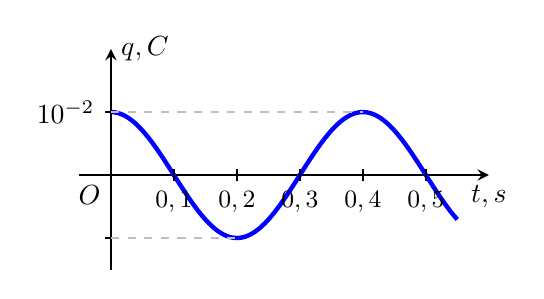
\begin{tikzpicture}[thick, scale=0.8, >=stealth]
    % Koordinata o'qlari
    \draw[->] (0,-1.5) -- (0,2) node[right] {$q, \text{C}$};
    \draw[->] (-0.5,0) -- (6,0) node[below] {$t, \text{s}$};
    \node[below left] at (0,0) {$O$};

    % Grafik (Kosinusoida)
    % Amplituda 1 birlik (10^-2), Davr 4 birlik (0.4 s)
    \draw[blue, ultra thick, domain=0:5.5, samples=100] plot (\x, {cos(\x*90)});

    % X-o'qidagi sonlar va belgilar
    \foreach \x/\val in {1/{0,1}, 2/{0,2}, 3/{0,3}, 4/{0,4}, 5/{0,5}} {
        \draw (\x, 0.1) -- (\x, -0.1) node[below, font=\small] {$\val$};
    }

    % Y-o'qidagi amplituda qiymati
    \draw (0.1, 1) -- (-0.1, 1) node[left] {$10^{-2}$};
    \draw (0.1, -1) -- (-0.1, -1);

    % Punktir yordamchi chiziqlar
    \draw[dashed, gray!50] (0,1) -- (4,1) (4,0);
    \draw[dashed, gray!50] (0,-1) -- (2,-1) (2,0);

\end{tikzpicture}

\begin{enumerate}[label=\Alph*)]
\item $q=10^{-2}\cos9\pi t$.
\item $q=10^{-2}\cos10\pi t$.
\item $q=10^{-2}\cos5\pi t$.
\item $q=10^{-2}\cos20\pi t$.
\item TJY.
\end{enumerate}

\item Tebranishlar konturidagi kondensatorning zaryadi $q=9\cdot10^{-5}\cos500t \ [\text{C}]$ qonun bo‘yicha o‘zgarmoqda. Agar kondensator sig‘imi $3~\mu$F bo‘lsa, kondensatordagi kuchlanishning maksimal qiymatini toping (V).
\begin{enumerate}[label=\Alph*)]
\item 15.
\item 30.
\item 90.
\item 60.
\item 10.
\end{enumerate}

\item Tebranishlar konturidagi zaryadning o‘zgarish qonuni $q=10^{-7}\cos10^6\pi t \ (\text{C})$ ko‘rinishga ega. Konturdagi tokning o‘zgarish chastotasini aniqlang (Hz).
\begin{enumerate}[label=\Alph*)]
\item $5\cdot10^5$.
\item $10^5$.
\item $10^{13}$.
\item $10^6$.
\item $2\cdot10^6$.
\end{enumerate}

\item Tebranishlar konturidagi zaryadning o‘zgarish qonuni $q=10^{-7}\cos10^6 t \ (\text{C})$ ko‘rinishga ega. Konturdagi tokning maksimal qiymatini toping (mA).
\begin{enumerate}[label=\Alph*)]
\item 1.
\item 5.
\item 10.
\item 100.
\item 1000.
\end{enumerate}

\item Konturda zaryad $q=10^{-3}\cos100\pi t$ qonun bo‘yicha tebranadi. Tokning amplituda qiymati qanday (mA)?
\begin{enumerate}[label=\Alph*)]
\item 0,1.
\item 1.
\item 3,14.
\item 31,4.
\item 314.
\end{enumerate}

\item Tebranishlar konturi kondensatoridagi zaryad $q=10^{-6}\sin(10^6t+\pi/3)\ (\text{C})$ qonun bo‘yicha o‘zgaradi. Konturdagi tok kuchining amplituda qiymati qanday (A)?
\begin{enumerate}[label=\Alph*)]
\item 0.
\item $10^{-6}$.
\item $10^{-2}$.
\item 0,1.
\item 1.
\end{enumerate}

\item Konturdagi zaryadning o‘zgarish tenglamasi $q=10^{-6}\cos10^6\pi t \ (\text{C})$ ko‘rinishga ega. Konturdagi tokning o‘zgarish qonunini yozing.
\begin{enumerate}[label=\Alph*)]
\item $i=10^{-6}\pi\sin10^6\pi t$.
\item $i=-\pi\sin10^6\pi t$.
\item $i=\cos10^6\pi t$.
\item $i=-10^{-6}\sin10^6\pi t$.
\item $i=10^{-6}\cos10^6\pi t$.
\end{enumerate}

\item Kuchlanish $u=220\cos100\pi t \ (\text{V})$ qonunga binoan o‘zgaradi. Kuchlanishning o‘zgarish davrini aniqlang(s).
\begin{enumerate}[label=\Alph*)]
\item 0,01.
\item 0,1.
\item 1.
\item 0,22.
\item 0,02.
\end{enumerate}

\item Elektr zanjiri qisqichlaridagi kuchlanish tebranishlari tenglamasi tuzilgan. Bunda kuchlanish tebranishlar amplitudasi $150$ V, davri $10^{-2}$ s, boshlang‘ich fazi nolga teng bo‘lib, $t=0$ momentda kuchlanish nolga teng deb hisoblang.
\begin{enumerate}[label=\Alph*)]
\item $u=150\sin100\pi t$.
\item $u=10^{-2}\sin150\pi t$.
\item $u=150\sin200\pi t$.
\item $u=10^{-2}\cos150\pi t$.
\item $u=150\cos100\pi t$.
\end{enumerate}

\item Kuchlanish $u=U\sin(\omega t+\pi/12)\ (\text{V})$ qonunga binoan o‘zgaradi. Agar $t=T/24$ vaqt momentidagi kuchlanish $50$ V bo‘lsa, kuchlanish amplitudasi qanday (V)?
\begin{enumerate}[label=\Alph*)]
\item 100.
\item 50.
\item 48.
\item 24.
\item 12.
\end{enumerate}

\item Tebranish konturidagi tok kuchining o‘zgarish qonuni $i=0,05\cos5\cdot10^6 t \ (\text{A})$ ko‘rinishiga ega. Konturdagi kondensator zaryadining maksimal qiymati qanday (nC)?
\begin{enumerate}[label=\Alph*)]
\item 5.
\item 10.
\item 25.
\item 50.
\item 25.
\end{enumerate}

\item Tebranishlar konturidagi tokning tebranishlar tenglamasi $i=4\pi\cdot10^{-3}\cos4\pi t \ (\text{A})$ ko‘rinishga ega. Bu kontur kondensatoridagi zaryad tebranishlar tenglamasini ko‘rsating.
\begin{enumerate}[label=\Alph*)]
\item $q=4\pi\cdot10^{-3}\sin4\pi t$.
\item $q=4\cdot10^{-3}\sin4\pi t$.
\item $q=4\cdot10^{-3}\cos4\pi t$.
\item $q=10^{-3}\sin4\pi t$.
\item $q=4\pi\cdot10^{-3}\cos4\pi t$.
\end{enumerate}

\item Tok kuchi vaqt bo‘yicha $i=5\cos200\pi t$ qonun bilan o‘zgaradi. Tok kuchi tebranishlarining chastotasi va davri qanday?
\begin{enumerate}[label=\Alph*)]
\item 100 Hz, 10 ms.
\item $100\pi$ Hz, 10 s.
\item $\pi$ Hz, $1/\pi$ s.
\item 100 Hz, 10 s.
\item TJY.
\end{enumerate}

\item O‘zgaruvchan tokning siklik chastotasi $1000\pi$ rad/s bo‘lsa, uning davri va chastotasi qanday?
\begin{enumerate}[label=\Alph*)]
\item 0,005 s; 200 Hz.
\item 0,002 s; 500 Hz.
\item 0,02 s; 50 Hz.
\item 0,001 s; 1000 Hz.
\item 0,01 s; 100 Hz.
\end{enumerate}

\item Tebranish konturidagi elektromagnit tebranishlar chastotasi $10^5$ Hz. Tebranishlar davri qanday ($\mu$s)?
\begin{enumerate}[label=\Alph*)]
\item $10^4$.
\item 1000.
\item 100.
\item 10.
\item 1.
\end{enumerate}

\item Tebranishlar konturi kondensatori zaryadining vaqtga bog‘lanish grafigi tasvirlangan. Zaryad tebranishlarining chastotasi necha Gers?

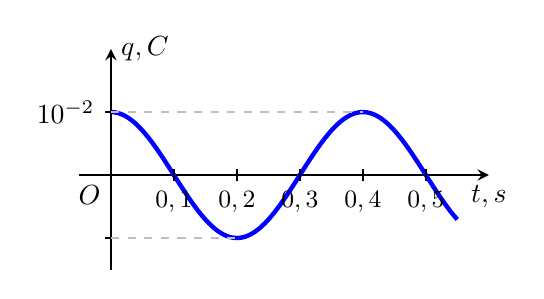
\begin{tikzpicture}[thick, scale=0.8, >=stealth]
    % Koordinata o'qlari
    \draw[->] (0,-1.5) -- (0,2) node[right] {$q, \text{C}$};
    \draw[->] (-0.5,0) -- (6,0) node[below] {$t, \text{s}$};
    \node[below left] at (0,0) {$O$};

    % Grafik (Kosinusoida)
    % Amplituda 1 birlik (10^-2), Davr 4 birlik (0.4 s)
    \draw[blue, ultra thick, domain=0:5.5, samples=100] plot (\x, {cos(\x*90)});

    % X-o'qidagi sonlar va belgilar
    \foreach \x/\val in {1/{0,1}, 2/{0,2}, 3/{0,3}, 4/{0,4}, 5/{0,5}} {
        \draw (\x, 0.1) -- (\x, -0.1) node[below, font=\small] {$\val$};
    }

    % Y-o'qidagi amplituda qiymati
    \draw (0.1, 1) -- (-0.1, 1) node[left] {$10^{-2}$};
    \draw (0.1, -1) -- (-0.1, -1);

    % Punktir yordamchi chiziqlar
    \draw[dashed, gray!50] (0,1) -- (4,1) (4,0);
    \draw[dashed, gray!50] (0,-1) -- (2,-1) (2,0);

\end{tikzpicture}

\begin{enumerate}[label=\Alph*)]
\item 5.
\item 2,5.
\item 3,3.
\item 10.
\item TJY.
\end{enumerate}

\item Tebranishlar konturi kondensatori qoplamalaridagi zaryadning amplituda qiymati $2,5\cdot10^{-6}$ C, tokning amplituda qiymati esa $3,14$ mA. Konturdagi elektromagnit tebranishlar chastotasi qanday?
\begin{enumerate}[label=\Alph*)]
\item 200 kHz.
\item 200 Hz.
\item 314 kHz.
\item 250 kHz.
\item 314 Hz.
\end{enumerate}

\end{enumerate}

\begin{table}[h!]
\centering
\begin{tabular}{|c|c|c|c|c|c|c|c|c|c|}
\hline
1d & 2d & 3c & 4e & 5c & 6a & 7d & 8b & 9a & 10d \\ \hline
11a & 12c & 13b & 14a & 15d & 16e & 17e & 18b & 19e & 20c \\ \hline
21a & 22b & 23d & 24a & 25b & 26d & 27b & 28b &  &  \\ \hline
\end{tabular}
\end{table}










\section{ Ideal tebranishlar konturi uchun Tomson formulasi.}

\begin{enumerate}

\item Ideal tebranishlar konturida hosil bo‘ladigan tebranishlarning davr formulasini ko‘rsating.
\begin{enumerate}[label=\Alph*)]
\item $T=2\pi\sqrt{LC}$.
\item $T=\sqrt{LC/2\pi}$.
\item $T=\sqrt{2\pi LC}$.
\item $T=2\pi\sqrt{LC}$.
\item $T=1/2\pi\sqrt{LC}$.
\end{enumerate}

\item Ideal tebranishlar konturida hosil bo‘ladigan tebranishlarning siklik chastotasi formulasini ko‘rsating.
\begin{enumerate}[label=\Alph*)]
\item $\omega=\sqrt{LC}$.
\item $\omega=\sqrt{L/C}$.
\item $\omega=\sqrt{C/L}$.
\item $\omega=LC$.
\item $\omega=1/\sqrt{LC}$.
\end{enumerate}

\item Tebranishlar konturi induktivligi $20$ mH bo‘lgan g‘altak va sig‘imi $200~\mu$F bo‘lgan kondensator tuzilgan bo‘lsa, unda hosil bo‘ladigan tebranishlar davri qanday bo‘ladi (ms).
\begin{enumerate}[label=\Alph*)]
\item $4\pi$.
\item $2\pi$.
\item $0,4$.
\item 2.
\item 1.
\end{enumerate}

\item Tebranishlar konturi sig‘imi va induktivligi $C=6~\mu$F va $L=5\cdot10^{-5}$ H. Konturdagi tebranishlar davrini toping ($\mu$s). $\pi\approx3$ deb hisoblansin.
\begin{enumerate}[label=\Alph*)]
\item 104.
\item 30.
\item 25.
\item 20.
\item 5.
\end{enumerate}

\item Tebranishlar konturi $2$ pF sig‘imli kondensator va induktivligi $0,5~\mu$H bo‘lgan g‘altakdan iborat. Konturdagi tebranishlar chastotasi qanday (MHz)?
\begin{enumerate}[label=\Alph*)]
\item 1,6.
\item 16.
\item 160.
\item 0,16.
\item 160 Hz.
\end{enumerate}

\item Induktivligi $L=1,5$ mH bo‘lgan g‘altakdan va sig‘imi $C=450$ pF bo‘lgan kondensatordan iborat konturdagi tebranishlar chastotasini aniqlang.
\begin{enumerate}[label=\Alph*)]
\item $0,2\cdot10^4$ Hz.
\item $2\cdot10^4$ Hz.
\item 20 kHz.
\item 2 MHz.
\item 0,2 MHz.
\end{enumerate}

\item Tebranish konturi induktivligi $1$ mH bo‘lgan g‘altak va sig‘imi $100$ nF bo‘lgan kondensatordan iborat. Bu konturning xususiy tebranishlarining siklik chastotasi qanday (rad/s)?
\begin{enumerate}[label=\Alph*)]
\item 100.
\item $10^3$.
\item $10^4$.
\item $10^5$.
\item 50.
\end{enumerate}

\item Tebranish konturi induktivligi $4$ marta oshirilsa, konturdagi tebranishlar chastotasi qanday o‘zgaradi?
\begin{enumerate}[label=\Alph*)]
\item o‘zgarmaydi.
\item 4 marta kamayadi.
\item 4 marta ortadi.
\item 2 marta ortadi.
\item 2 marta kamayadi.
\end{enumerate}

\item Kondensatorning elektr sig‘imi $2$ marta ortganda, tebranishlar konturidagi erkin tebranishlar davri qanday o‘zgaradi?
\begin{enumerate}[label=\Alph*)]
\item $\sqrt2$ marta ortadi.
\item $\sqrt2$ marta kamayadi.
\item 2 marta ortadi.
\item 2 marta kamayadi.
\item TJY.
\end{enumerate}

\item Tebranishlar konturining induktivligini va sig‘imini $4$ marta oshirsak, konturdagi tebranishlar davri qanday o‘zgaradi?
\begin{enumerate}[label=\Alph*)]
\item o‘zgarmay qoladi.
\item 4 marta kamayadi.
\item 16 marta oshadi.
\item 16 marta kamayadi.
\item 4 marta oshadi.
\end{enumerate}

\item Tebranishlar konturidagi tebranishlar davri qanday hollarda oshadi?
\begin{enumerate}[label=\Alph*)]
\item 1, 2, 3.
\item 2, 4.
\item 1, 4.
\item 1, 3.
\item 4.
\end{enumerate}

\item $C=6~\mu$F va $L=5\cdot10^{-5}$ H bo‘lsa, konturdagi tebranishlar davri qanday ($\mu$s)? $\pi\approx3$.

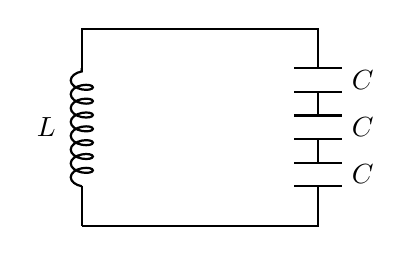
\begin{tikzpicture}[thick, scale=1]
    % Kontur asosiy ramkasi
    \draw (0,0) -- (0,0.5);
    \draw (0,2) -- (0,2.5) -- (3,2.5) -- (3,2);
    \draw (3,1.7)--(3,1.4);
     \draw (3,0.8)--(3,1.1);
    \draw (3,0.5) -- (3,0) -- (0,0);

    % G'altak (L) - chap tomonda
    \draw[decoration={coil, aspect=0.5, segment length=5pt, amplitude=4pt}, decorate] (0, 0.5) -- (0, 2);
    \node[left] at (-0.2, 1.25) {$L$};

    
    \draw (2.7, 1.1) -- (3.3, 1.1) (2.7, 1.4) -- (3.3, 1.4);
    \draw (2.7, 1.7) -- (3.3, 1.7) (2.7, 2) -- (3.3, 2);
    \draw (2.7, 0.5) -- (3.3, 0.5) (2.7, 0.8) -- (3.3, 0.8);


    
    \node[right] at (3.3, 1.85) {$C$};
     \node[right] at (3.3, 1.25) {$C$};
      \node[right] at (3.3, 0.65) {$C$};

\end{tikzpicture}

\begin{enumerate}[label=\Alph*)]
\item 60.
\item 30.
\item 25.
\item 20.
\item 5.
\end{enumerate}

\item $C=1~\mu$F va $L=3\cdot10^{-4}$ H bo‘lsa, konturdagi tebranishlar davri qanday ($\mu$s)? $\pi\approx3$ deb hisoblansin.

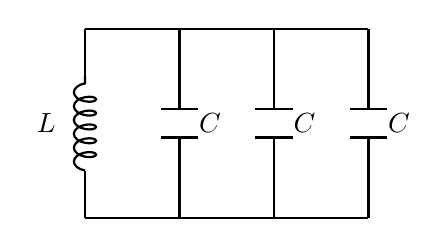
\begin{tikzpicture}[thick, scale=1.2]
    % Gorizontal ulovchi simlar (relslar)
    \draw (0,2) -- (3,2);
    \draw (0,0) -- (3,0);

    % Induktivlik g'altagi L (chapda)
    \draw[decoration={coil, aspect=0.5, segment length=5pt, amplitude=4pt}, decorate] (0, 0.5) -- (0, 1.5);
    \draw (0,2) -- (0,1.5);
    \draw (0,0) -- (0,0.5);
    \node[left] at (-0.2, 1) {$L$};

    % 1-kondensator C
    \draw (1, 2) -- (1, 1.15);
    \draw (1, 0) -- (1, 0.85);
    \draw (0.8, 1.15) -- (1.2, 1.15);
    \draw (0.8, 0.85) -- (1.2, 0.85);
    \node[right] at (1.1, 1) {$C$};

    % 2-kondensator C
    \draw (2, 2) -- (2, 1.15);
    \draw (2, 0) -- (2, 0.85);
    \draw (1.8, 1.15) -- (2.2, 1.15);
    \draw (1.8, 0.85) -- (2.2, 0.85);
    \node[right] at (2.1, 1) {$C$};

    % 3-kondensator C
    \draw (3, 2) -- (3, 1.15);
    \draw (3, 0) -- (3, 0.85);
    \draw (2.8, 1.15) -- (3.2, 1.15);
    \draw (2.8, 0.85) -- (3.2, 0.85);
    \node[right] at (3.1, 1) {$C$};

\end{tikzpicture}

\begin{enumerate}[label=\Alph*)]
\item 18.
\item 54.
\item 60.
\item 90.
\item 180.
\end{enumerate}

\item Chizmada tasvirlangan konturdagi elektromagnit tebranishlar davrini toping.

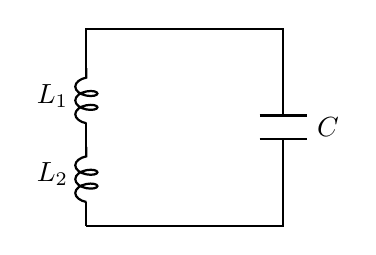
\begin{tikzpicture}[thick, scale=1]
    % Kontur asosiy ramkasi
    \draw (0,0) -- (0,0.3);
    \draw (0,1) -- (0,1.3);
    \draw (0,2) -- (0,2.5) -- (2.5,2.5) -- (2.5,1.4);
    \draw (2.5,1.1) -- (2.5,0) -- (0,0);

    % 1-g'altak (L1)
    \draw[decoration={coil, aspect=0.5, segment length=5pt, amplitude=4pt}, decorate] (0, 1.3) -- (0, 2);
    \node[left] at (-0.1, 1.65) {$L_1$};

    % 2-g'altak (L2)
    \draw[decoration={coil, aspect=0.5, segment length=5pt, amplitude=4pt}, decorate] (0, 0.3) -- (0, 1);
    \node[left] at (-0.1, 0.65) {$L_2$};

    % Kondensator (C)
    \draw (2.2, 1.1) -- (2.8, 1.1) (2.2, 1.4) -- (2.8, 1.4);
    \node[right] at (2.8, 1.25) {$C$};

\end{tikzpicture}

\begin{enumerate}[label=\Alph*)]
\item $T=2\pi\sqrt{2(L_1+L_2)C}$.
\item $T=2\pi\sqrt{(L_1+L_2)C/2}$.
\item $T=2\pi\sqrt{(L_1+L_2)C}$.
\item $T=4\pi\sqrt{(L_1+L_2)C}$.
\item $T=2\pi\sqrt{|L_1-L_2|C}$.
\end{enumerate}

\item Chizmada tasvirlangan konturdagi elektromagnit tebranishlar davrini toping.

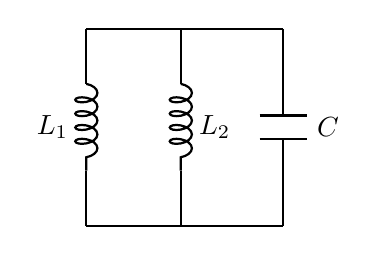
\begin{tikzpicture}[thick, scale=1]
    % Konturning gorizontal ulovchi simlari
    \draw (0,2.5) -- (2.5,2.5);
    \draw (0,0) -- (2.5,0);

    % 1-g'altak (L1) - chapki tarmoqda
    \draw (0,2.5) -- (0,1.8);
    \draw[decoration={coil, aspect=0.5, segment length=5pt, amplitude=4pt}, decorate] (0, 1.8) -- (0, 0.7);
    \draw (0,0.7) -- (0,0);
    \node[left] at (-0.1, 1.25) {$L_1$};

    % 2-g'altak (L2) - o'rta tarmoqda (L1 ga parallel)
    \draw (1.2,2.5) -- (1.2,1.8);
    \draw[decoration={coil, aspect=0.5, segment length=5pt, amplitude=4pt}, decorate] (1.2, 1.8) -- (1.2, 0.7);
    \draw (1.2,0.7) -- (1.2,0);
    \node[right] at (1.3, 1.25) {$L_2$};

    % Kondensator (C) - o'ngki tarmoqda
    \draw (2.5,2.5) -- (2.5,1.4);
    \draw (2.5,0) -- (2.5,1.1);
    \draw (2.2, 1.4) -- (2.8, 1.4);
    \draw (2.2, 1.1) -- (2.8, 1.1);
    \node[right] at (2.8, 1.25) {$C$};

\end{tikzpicture}

\begin{enumerate}[label=\Alph*)]
\item $T=2\pi\sqrt{(L_1+L_2)C}$.
\item $T=2\pi\sqrt{|L_1-L_2|C}$.
\item $T=2\pi\sqrt{\dfrac{L_1L_2}{L_1+L_2}C}$.
\item $T=2\pi\sqrt{\dfrac{2L_1L_2}{L_1+L_2}C}$.
\item $T=4\pi\sqrt{(L_1+L_2)C}$.
\end{enumerate}

\item a-sxemadan b-sxemaga o‘tganda tebranishlar konturidagi erkin elektromagnit tebranishlar davri qanday o‘zgaradi?

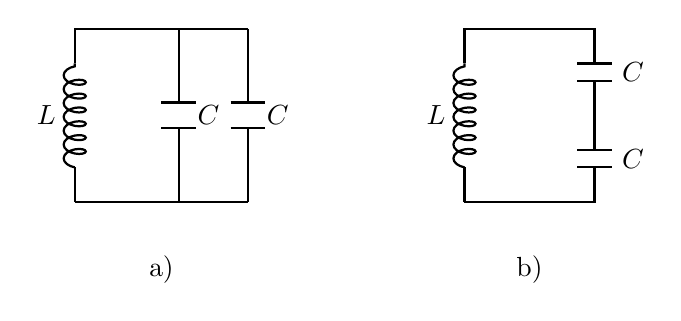
\begin{tikzpicture}[thick, scale=1.1]

    % --- a-sxema (Parallel ulanish) ---
    \begin{scope}[xshift=0cm]
        \draw (0,0) -- (0,0.4);
        \draw (0,1.6) -- (0,2) -- (2,2);
        \draw (0,0) -- (2,0);
        
        % G'altak L
        \draw[decoration={coil, aspect=0.5, segment length=5pt, amplitude=4pt}, decorate] (0, 0.4) -- (0, 1.6);
        \node[left] at (-0.1, 1) {$L$};

        % Kondensator 1
        \draw (1.2, 2) -- (1.2, 1.15) (1.2, 0.85) -- (1.2, 0);
        \draw (1, 1.15) -- (1.4, 1.15) (1, 0.85) -- (1.4, 0.85);
        \node[right] at (1.3, 1) {$C$};

        % Kondensator 2
        \draw (2, 2) -- (2, 1.15) (2, 0.85) -- (2, 0);
        \draw (1.8, 1.15) -- (2.2, 1.15) (1.8, 0.85) -- (2.2, 0.85);
        \node[right] at (2.1, 1) {$C$};
        
        \node[below] at (1, -0.5) {a)};
    \end{scope}

    % --- b-sxema (Ketma-ket ulanish) ---
    \begin{scope}[xshift=4.5cm]
        \draw (0,0) -- (0,0.4);
        \draw (0,1.6) -- (0,2) -- (1.5,2) -- (1.5,1.6);
        \draw (0,0) -- (1.5,0) -- (1.5,0.4);
        
        % G'altak L
        \draw[decoration={coil, aspect=0.5, segment length=5pt, amplitude=4pt}, decorate] (0, 0.4) -- (0, 1.6);
        \node[left] at (-0.1, 1) {$L$};

        % Ketma-ket kondensatorlar
        \draw (1.3, 1.6) -- (1.7, 1.6) (1.3, 1.4) -- (1.7, 1.4); % C1
        \draw (1.5, 1.4) -- (1.5, 0.6);
        \draw (1.3, 0.6) -- (1.7, 0.6) (1.3, 0.4) -- (1.7, 0.4); % C2
        
        \node[right] at (1.7, 1.5) {$C$};
        \node[right] at (1.7, 0.5) {$C$};
        
        \node[below] at (0.75, -0.5) {b)};
    \end{scope}

\end{tikzpicture}

\begin{enumerate}[label=\Alph*)]
\item 2 marta kamayadi.
\item 4 marta ortadi.
\item 2 marta ortadi.
\item 4 marta kamayadi.
\item o‘zgarmaydi.
\end{enumerate}

\item a-sxemadan b-sxemaga o‘tganda, tebranishlar konturidagi erkin elektromagnit tebranishlar chastotasi qanday o‘zgaradi?

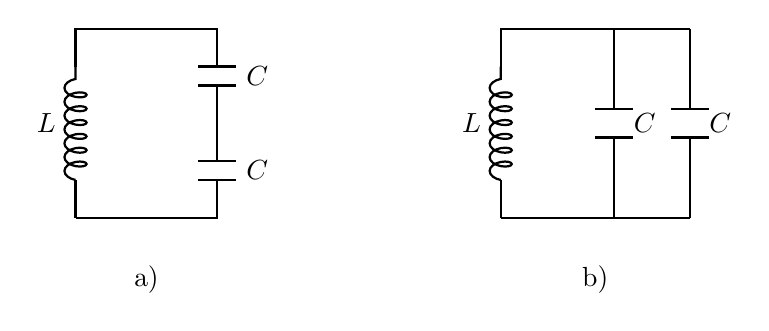
\begin{tikzpicture}[thick, scale=1.2]

    % --- a-sxema (Kondensatorlar parallel) ---
    \begin{scope}[xshift=4.5cm]
        \draw (0,0) -- (0,0.4);
        \draw (0,1.6) -- (0,2) -- (2,2);
        \draw (0,0) -- (2,0);
        
        % G'altak L
        \draw[decoration={coil, aspect=0.5, segment length=5pt, amplitude=4pt}, decorate] (0, 0.4) -- (0, 1.6);
        \node[left] at (-0.1, 1) {$L$};

        % 1-kondensator C
        \draw (1.2, 2) -- (1.2, 1.15) (1.2, 0.85) -- (1.2, 0);
        \draw (1, 1.15) -- (1.4, 1.15) (1, 0.85) -- (1.4, 0.85);
        \node[right] at (1.3, 1) {$C$};

        % 2-kondensator C
        \draw (2, 2) -- (2, 1.15) (2, 0.85) -- (2, 0);
        \draw (1.8, 1.15) -- (2.2, 1.15) (1.8, 0.85) -- (2.2, 0.85);
        \node[right] at (2.1, 1) {$C$};
        
        \node[below] at (1, -0.4) {b)};
    \end{scope}

    % --- b-sxema (Kondensatorlar ketma-ket) ---
    \begin{scope}
        \draw (0,0) -- (0,0.4);
        \draw (0,1.6) -- (0,2) -- (1.5,2) -- (1.5,1.6);
        \draw (0,0) -- (1.5,0) -- (1.5,0.4);
        
        % G'altak L
        \draw[decoration={coil, aspect=0.5, segment length=5pt, amplitude=4pt}, decorate] (0, 0.4) -- (0, 1.6);
        \node[left] at (-0.1, 1) {$L$};

        % Ketma-ket ulanish
        \draw (1.3, 1.6) -- (1.7, 1.6) (1.3, 1.4) -- (1.7, 1.4); % C yuqori
        \draw (1.5, 1.4) -- (1.5, 0.6);
        \draw (1.3, 0.6) -- (1.7, 0.6) (1.3, 0.4) -- (1.7, 0.4); % C pastki
        
        \node[right] at (1.7, 1.5) {$C$};
        \node[right] at (1.7, 0.5) {$C$};
        
        \node[below] at (0.75, -0.4) {a)};
    \end{scope}

\end{tikzpicture}

\begin{enumerate}[label=\Alph*)]
\item 4 marta kamayadi.
\item 2 marta oshadi.
\item o‘zgarmaydi.
\item 4 marta oshadi.
\item 2 marta kamayadi.
\end{enumerate}

\item Sig‘imi $100~\mu$F bo‘lgan kondensator va induktivligi $10~\mu$H bo‘lgan g‘altakdan tashkil topgan tebranish konturida 1 min da nechta elektr tebranishlari yuzaga keladi? $(\pi^2=10)$.
\begin{enumerate}[label=\Alph*)]
\item $10^5$.
\item $3\cdot10^5$.
\item $90\cdot10^5$.
\item $60\cdot10^5$.
\item $9\cdot10^5$.
\end{enumerate}

\item Agar ideal tebranish konturidagi $C$ sig‘imli kondensatorga $3C$ sig‘imli kondensator parallel ulansa, undagi erkin elektromagnit tebranishlar davri qanday o‘zgaradi?
\begin{enumerate}[label=\Alph*)]
\item 2 marta kamayadi.
\item 2 marta oshadi.
\item o‘zgarmaydi.
\item 3 marta kamayadi.
\item 3 marta oshadi.
\end{enumerate}

\item Tebranishlar konturidagi $C$ sig‘imli kondensatorga $3C$ sig‘imli kondensator parallel ulansa, undagi erkin elektromagnit tebranishlar chastotasi qanday o‘zgaradi?
\begin{enumerate}[label=\Alph*)]
\item 2 marta oshadi.
\item 4 marta kamayadi.
\item 2 marta kamayadi.
\item 4 marta oshadi.
\item o‘zgarmaydi.
\end{enumerate}

\item Tebranishlar konturidagi $C$ sig‘imli kondensatorga $C/3$ sig‘imli kondensator ketma-ket ulansa, undagi erkin elektromagnit tebranishlar davri qanday o‘zgaradi?
\begin{enumerate}[label=\Alph*)]
\item 2 marta oshadi.
\item 2 marta kamayadi.
\item o‘zgarmaydi.
\item 3 marta kamayadi.
\item 3 marta oshadi.
\end{enumerate}

\item Tebranishlar konturidagi $C$ sig‘imli kondensatorga $C/3$ sig‘imli kondensator ketma-ket ulansa, undagi erkin elektromagnit tebranishlar chastotasi qanday o‘zgaradi?
\begin{enumerate}[label=\Alph*)]
\item 3 marta kamayadi.
\item 3 marta oshadi.
\item 2 marta oshadi.
\item 2 marta kamayadi.
\item o‘zgarmaydi.
\end{enumerate}

\item Tebranishlar konturidagi yassi havo kondensatori plastinalari orasidagi masofa $25$ marta ortirilsa, konturdagi erkin elektromagnit tebranishlar davri qanday o‘zgaradi?
\begin{enumerate}[label=\Alph*)]
\item 5 marta ortadi.
\item 5 marta kamayadi.
\item 25 marta ortadi.
\item 25 marta kamayadi.
\item TJY.
\end{enumerate}

\item Tebranishlar konturidagi yassi havo kondensatori plastinalari orasidagi masofa $7$ marta ortirilsa, tebranishlar chastotasi qanday o‘zgaradi?
\begin{enumerate}[label=\Alph*)]
\item o‘zgarmaydi.
\item 7 marta ortadi.
\item 7 marta kamayadi.
\item $\sqrt7$ marta ortadi.
\item $\sqrt7$ marta kamayadi.
\end{enumerate}

\item Konturdagi kondensator ichiga $\varepsilon=6,25$ bo‘lgan dielektrik kiritilsa, undagi elektromagnit tebranishlar davri qanday o‘zgaradi?
\begin{enumerate}[label=\Alph*)]
\item o‘zgarmaydi.
\item 6,25 marta oshadi.
\item 6,25 marta kamayadi.
\item 2,5 marta oshadi.
\item 2,5 marta kamayadi.
\end{enumerate}

\item Tebranishlar konturidagi havo kondensatorining qoplamalari orasiga dielektrik singdiruvchanligi $\varepsilon=3,24$ bo‘lgan dielektrik modda kiritilsa, konturdagi tebranishlar chastotasi qanday o‘zgaradi?
\begin{enumerate}[label=\Alph*)]
\item o‘zgarmaydi.
\item 1,8 marta kamayadi.
\item 3,24 marta ortadi.
\item 3,24 marta kamayadi.
\item 1,8 marta ortadi.
\end{enumerate}

\item Tebranishlar konturidagi g‘altak ichiga ferromagnitdan yasalgan o‘zak kiritilsa, elektromagnit tebranishlar chastotasi qanday o‘zgaradi?
\begin{enumerate}[label=\Alph*)]
\item ortadi.
\item avval ortib, keyin kamayadi.
\item kamayadi.
\item avval kamayib, keyin ortadi.
\item o‘zgarmaydi.
\end{enumerate}

\item Induktivligi $12,5$ mH bo‘lgan tebranish konturiga qanday sig‘imli kondensator ulansa, uning chastotasi $10^3$ Hz bo‘ladi ($\mu$F)?
\begin{enumerate}[label=\Alph*)]
\item 2.
\item 3.
\item 5.
\item 20.
\item 30.
\end{enumerate}

\item Tebranish konturida davri $1$ ms bo‘lgan tebranish hosil qilish uchun induktivligi $20$ mH bo‘lgan g‘altakka qanday sig‘imli ($\mu$F) kondensator ulash kerak? $\pi^2=10$.
\begin{enumerate}[label=\Alph*)]
\item 125.
\item 12,5.
\item 5.
\item 2,5.
\item 1,25.
\end{enumerate}

\item Tebranish konturidagi erkin tebranishlar chastotasi $50$ Hz. Kondensator sig‘imi $20$ nF. G‘altak induktivligi qanday (H)? $\pi^2=10$.
\begin{enumerate}[label=\Alph*)]
\item 0,5.
\item 1.
\item 2,5.
\item 0,5.
\item 10.
\end{enumerate}

\item Ideal tebranishlar konturidagi kondensatorning sig‘imi $4~\mu$F, tebranishlarning siklik chastotasi $500$ rad/s bo‘lsa, g‘altakning induktivligi necha Genri?
\begin{enumerate}[label=\Alph*)]
\item 0,05.
\item 0,1.
\item 0,5.
\item 0,8.
\item 1.
\end{enumerate}

\item Tebranishlar konturidagi induktivligi g‘altak ichiga temir o‘zak kiritilsa, kondensatordagi kuchlanish tebranishlari davri va amplitudasi qanday o‘zgaradi?
\begin{enumerate}[label=\Alph*)]
\item davri va amplitudasi ortadi.
\item davri ortadi, amplitudasi o‘zgarmaydi.
\item davri kamayadi, amplitudasi ortadi.
\item davri o‘zgarmaydi, amplitudasi ortadi.
\item davri kamayadi, amplitudasi kamayadi.
\end{enumerate}

\item Tebranishlar konturi sig‘imi $2~\mu$F bo‘lgan kondensator va induktivligi $2$ H bo‘lgan g‘altakdan tuzilgan bo‘lib, kondensatorga $200~\mu$C zaryad berildi. Konturda hosil bo‘ladigan elektr tok tebranishlari tenglamasini yozing.
\begin{enumerate}[label=\Alph*)]
\item $i=-0,05\sin250t$.
\item $i=200\sin16t$.
\item $i=-0,1\sin500t$.
\item $i=16\sin200t$.
\item $i=-0,5\sin200t$.
\end{enumerate}

\item Tebranish konturidagi tok $i=0,01\cos1000t$ qonun bo‘yicha o‘zgaradi. Undagi kondensatorning sig‘imi $2\cdot10^{-5}$ F bo‘lsa, konturning induktivligi qanday (mH)?
\begin{enumerate}[label=\Alph*)]
\item 5.
\item 20.
\item 25.
\item 50.
\item 70.
\end{enumerate}

\item Rasmda ko‘rsatilgan zanjirdagi g‘altakning induktivligi $0,2$ H, kondensator sig‘imi $8\cdot10^{-3}$ F va $0,01$ C gacha zaryadlangan. Agar K kalit ulansa, zanjirdagi tok kuchining o‘zgarish qonuni qanday ko‘rinishda bo‘ladi?

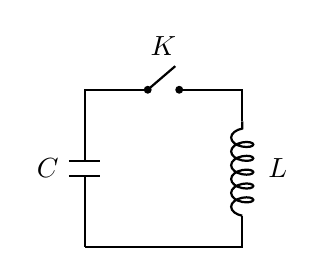
\begin{tikzpicture}[thick, scale=1]
    % Kontur ramkasi
    \draw (0,0) -- (2,0) -- (2,0.4);
    \draw (2,1.6) -- (2,2) -- (1.2,2);
    \draw (0.8,2) -- (0,2) -- (0,1.1);
    \draw (0,0.9) -- (0,0);

    % Kondensator (C) - chap tomonda
    \draw (-0.2, 0.9) -- (0.2, 0.9);
    \draw (-0.2, 1.1) -- (0.2, 1.1);
    \node[left] at (-0.2, 1) {$C$};

    % Kalit (K) - yuqori tomonda (ochiq holatda)
    \draw (0.8, 2) -- (1.15, 2.3);
    \filldraw (0.8, 2) circle (1pt);
    \filldraw (1.2, 2) circle (1pt);
    \node[above] at (1, 2.3) {$K$};

    % G'altak (L) - o'ng tomonda
    \draw[decoration={coil, aspect=0.5, segment length=5pt, amplitude=4pt}, decorate] (2, 0.4) -- (2, 1.6);
    \node[right] at (2.2, 1) {$L$};

\end{tikzpicture}

\begin{enumerate}[label=\Alph*)]
\item $i=-0,25\sin25t$.
\item $i=-0,01\sin25t$.
\item $i=-0,25\sin40t$.
\item $i=-0,04\sin40t$.
\item $i=-0,01\sin1,6t$.
\end{enumerate}

\item Erkin elektromagnit tebranishlar sodir bo‘layotgan tebranishlar konturidagi tok kuchi $i=0,2\cos10^6 t$ (A) qonuniyat bo‘yicha o‘zgaradi. Agar konturdagi g‘altak induktivligi $2$ mH bo‘lsa, kondensator sig‘imi qanday (pF)?
\begin{enumerate}[label=\Alph*)]
\item 500.
\item 1000.
\item 20.
\item 200.
\item 10000.
\end{enumerate}

\end{enumerate}

\begin{table}[h!]
\centering
\begin{tabular}{|c|c|c|c|c|c|c|c|c|c|}
\hline
1d & 2e & 3a & 4a & 5c & 6e & 7d & 8d & 9a & 10e \\ \hline
11d & 12a & 13e & 14c & 15c & 16a & 17e & 18b & 19b & 20c \\ \hline
21b & 22c & 23b & 24d & 25d & 26b & 27c & 28a & 29e & 30a \\ \hline
31e & 32b & 33c & 34d & 35a & 36a &  &  &  &  \\ \hline
\end{tabular}
\end{table}



\section{Tebranishlar konturida energiya.}


\begin{enumerate}

\item Kuzatish boshlangan vaqtda ideal tebranish konturidagi elektr maydon energiyasi $6$ mJ, magnit maydon energiyasi $8$ mJ bo‘lgan. Sistemaning to‘la energiyasini (mJ) aniqlang.
\begin{enumerate}[label=\Alph*)]
\item 48.
\item 14.
\item 10.
\item 5.
\item 2.
\end{enumerate}

\item Tebranish jarayonida elektromagnit tebranishlar konturida qanday fizik kattaliklar bir-biriga aylanadi?
\begin{enumerate}[label=\Alph*)]
\item tok kuchi va potensiallar ayirmasi.
\item potensial va kinetik energiyalar.
\item zaryadlar va toklar.
\item induktivlik va sig‘im.
\item elektr va magnit maydonlar energiyalari.
\end{enumerate}

\item Tebranish konturidagi kondensatorning sig‘imi $C=200$ nF, g‘altakning induktivligi $L=5$ H. Kondensator zaryadining oniy qiymati $q=60~\mu$C bo‘lgan paytda konturdagi tok kuchining oniy qiymati $i=40$ mA bo‘lgan. Konturdagi to‘la elektromagnit maydon energiyasi nimaga teng (mJ)?
\begin{enumerate}[label=\Alph*)]
\item 10.
\item 13.
\item 18.
\item 14.
\item 21.
\end{enumerate}

\item Tebranishlar konturidagi kondensator sig‘imi $C=80~\mu$F, g‘altakning induktivligi $L=8$ H. Kondensator kuchlanishining oniy qiymati $u=25$ V bo‘lgan paytda, konturdagi tok kuchining oniy qiymati $i=20$ mA bo‘lgan. Konturdagi to‘la elektromagnit maydon energiyasi nimaga teng (mJ)?
\begin{enumerate}[label=\Alph*)]
\item 26,6.
\item 55,1.
\item 45,9.
\item 39,5.
\item 34,8.
\end{enumerate}

\item Tebranish konturidagi $2~\mu$F sig‘imli kondensator qoplamalariga $4\cdot10^{-3}$ C maksimal zaryadlangan. Konturdagi to‘la elektromagnit maydon energiyasi nimaga teng(J)?
\begin{enumerate}[label=\Alph*)]
\item 4000.
\item 2000.
\item 40.
\item 4.
\item 2.
\end{enumerate}

\item Tebranishlar konturidagi g‘altakning induktivligi $2,8$ H, konturdagi tok kuchining amplituda qiymati $5$ A. Konturdagi to‘la elektromagnit maydon energiyasi nimaga teng(J)?
\begin{enumerate}[label=\Alph*)]
\item 4.
\item 12.
\item 44.
\item 25.
\item 35.
\end{enumerate}

\item Berilganlar ichidan energiyaning saqlanish qonuni ifodasini toping:
\begin{enumerate}
\item $m_1v_1+m_2v_2=m_1u_1+m_2u_2$;
\item $E=mgh_2-mgh_1$;
\item $E=E_k+E_p=\mathrm{const}$;
\item $E=\dfrac{mv_2^2}{2}-\dfrac{mv_1^2}{2}$;
\item $E=\dfrac{Li^2}{2}+\dfrac{q^2}{2C}=\mathrm{const}$.
\end{enumerate}
\begin{enumerate}[label=\Alph*)]
\item 3; 5.
\item 2; 4.
\item 1; 3.
\item 4.
\item 5.
\end{enumerate}

\item Ideal tebranishlar konturidagi garmonik tebranishlar vaqtida g‘altak magnit maydoni energiyasining maksimal qiymati $20$ J ga teng bo‘lsa, kondensator elektr maydoni energiyasining maksimal qiymati necha Joulga teng bo‘ladi?
\begin{enumerate}[label=\Alph*)]
\item 5.
\item 8.
\item 10.
\item 20.
\item 40.
\end{enumerate}

\item Ideal tebranish konturidagi kondensatorda elektr maydonning maksimal energiyasi $18$ J bo‘lsa, konturdagi elektromagnit tebranish energiyasi vaqt bo‘yicha qanday o‘zgaradi?
\begin{enumerate}[label=\Alph*)]
\item o‘zgarmaydi va $36$ J ga teng.
\item 0 dan 18 J gacha.
\item o‘zgarmaydi va 18 J ga teng.
\item 0 dan 36 J gacha.
\item o‘zgarmaydi va 6 J ga teng.
\end{enumerate}

\item Aktiv qarshiliksiz tebranish konturi kondensatorining zaryadi rasmda ko‘rsatilgandek o‘zgarsa, paytda kontur elektromagnit maydoni energiyasi nimaga teng?

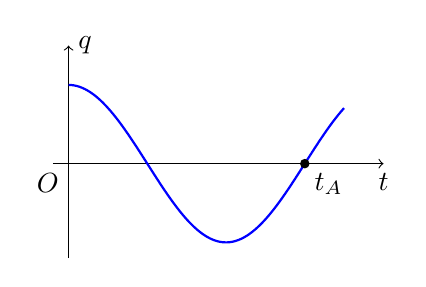
\begin{tikzpicture}
    % Koordinata o'qlari
    \draw[->] (0,-1.2) -- (0,1.5) node[right] {$q$};
    \draw[->] (-0.2,0) -- (4,0) node[below] {$t$};
    \node[below left] at (0,0) {$O$};

    % Grafik (Kosinusoida shaklida zaryad o'zgarishi)
    % q = q_m * cos(wt)
    \draw[blue, thick, domain=0:3.5, samples=100] plot (\x, {cos(\x*90)});

    % t_A nuqtasi (Zaryad nolga teng bo'lgan moment)
    % Grafik 3-marta o'qni kesib o'tgan nuqtada (yoki savolga ko'ra belgilangan nuqtada)
    \filldraw (3,0) circle (1.5pt);
    \node[below right] at (3,0) {$t_A$};

    % Amplituda belgilari (ixtiyoriy)
    %\draw[dashed, gray] (0,1) -- (0.5,1);
    %\node[left] at (0,1) {$q_m$};

\end{tikzpicture}

\begin{enumerate}[label=\Alph*)]
\item 0.
\item $LI_m^2/2$.
\item $q_m^2/2C$.
\item $q^2/C+LI^2/2$.
\item aniqlab bo‘lmaydi.
\end{enumerate}

\item Aktiv qarshiliksiz tebranish konturidagi tok kuchi rasmda ko‘rsatilgandek o‘zgarsa, paytda kontur elektromagnit maydoni energiyasi nimaga teng?

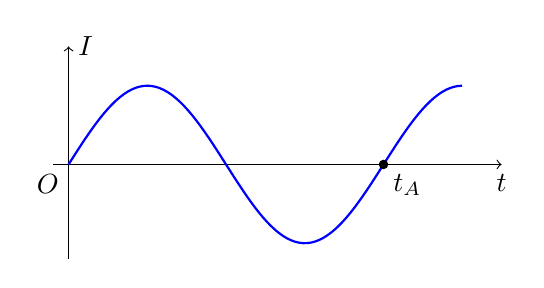
\begin{tikzpicture}
    % Koordinata o'qlari
    \draw[->] (0,-1.2) -- (0,1.5) node[right] {$I$};
    \draw[->] (-0.2,0) -- (5.5,0) node[below] {$t$};
    \node[below left] at (0,0) {$O$};

    % Grafik (Sinusoida shaklida tok o'zgarishi)
    % I = I_m * sin(wt)
    \draw[blue, thick, domain=0:5, samples=100] plot (\x, {sin(\x*90)});

   
    \filldraw (4,0) circle (1.5pt); 
    
    % Savoldagi rasmga ko'ra t_A nuqtasi (T davrda)
    \node[below right] at (4,0) {$t_A$};

\end{tikzpicture}

\begin{enumerate}[label=\Alph*)]
\item 0.
\item $LI^2/2$.
\item $LI_m^2/2$.
\item $q_m^2/2C$.
\item aniqlab bo‘lmaydi.
\end{enumerate}

\item Tebranishlar konturidagi kondensator sig‘imi $5~\mu$F, undagi zaryad $q=2\cdot10^{-5}\cos10^5\pi t$ (C) qonun bo‘yicha o‘zgaryapti. Konturdagi magnit maydon energiyasining maksimal qiymatini toping ($\mu$J).
\begin{enumerate}[label=\Alph*)]
\item 40.
\item 50.
\item 200.
\item 20.
\item 5.
\end{enumerate}

\item Tebranish konturi kondensatoridagi kuchlanishning o‘zgarishi $u=10\cos(2\cdot10^{-3}\pi t)$ (V) qonun bilan berilgan. Kondensator sig‘imi $2,6\cdot10^{-2}~\mu$F. Konturdagi magnit maydon energiyasining maksimal qiymati qanday (J)?
\begin{enumerate}[label=\Alph*)]
\item $2,6\cdot10^{-6}$.
\item $0,65\cdot10^{-6}$.
\item $1,3\cdot10^{-6}$.
\item $2,6\cdot10^{-4}$.
\item $1,3\cdot10^{-4}$.
\end{enumerate}

\item Tebranish konturidagi g‘altak induktivligi $10$ mH, undagi tok $i=0,05\cos10^5\pi t$ (A) qonun bo‘yicha o‘zgaryapti. Kontur elektr maydoni energiyasining maksimal qiymatini toping ($\mu$J).
\begin{enumerate}[label=\Alph*)]
\item 12,5.
\item 50.
\item 25.
\item 50.
\item 125.
\end{enumerate}

\item Tebranish konturining kondensatori to‘la zaryadlangan paytda konturdagi tok kuchi qanday bo‘ladi (A)? G‘altakning magnit maydon maksimal energiyasi $2\cdot10^{-4}$ J, uning induktivligi $1$ H.
\begin{enumerate}[label=\Alph*)]
\item 0,04.
\item 0,2.
\item 0,4.
\item 0.
\item 0.
\end{enumerate}

\item Kondensator to‘la razryadsizlangan paytda tebranishlar konturidagi tok kuchi necha Amperga teng bo‘ladi? G‘altak induktivligi $5$ H, magnit maydon maksimal energiyasi $28,9$ J.
\begin{enumerate}[label=\Alph*)]
\item 1,4.
\item 2,4.
\item 3,4.
\item 4,4.
\item 5,4.
\end{enumerate}

\item Sig‘imi $40~\mu$F bo‘lgan kondensator $200$ V kuchlanishga zaryadlangan va induktivligi $0,1$ H bo‘lgan g‘altakka ulangan. G‘altakdagi tok kuchining maksimal qiymati qanday (A)?
\begin{enumerate}[label=\Alph*)]
\item 0,2.
\item 0,4.
\item 2.
\item 4.
\item 20.
\end{enumerate}

\item Zaryadi $10^{-5}$ C, sig‘imi $5~\mu$F bo‘lgan kondensator induktivligi $50$ mH bo‘lgan g‘altakka ulangandagi tokning maksimal qiymatini toping(mA).
\begin{enumerate}[label=\Alph*)]
\item 20.
\item 10.
\item 5.
\item 2.
\item 1.
\end{enumerate}

\item Tebranish konturi sig‘imi $2500$ pF bo‘lgan kondensator va induktivligi $10$ mH bo‘lgan g‘altakdan iborat. Agar kondensatordagi kuchlanishning maksimal qiymati $200$ V bo‘lsa, tok kuchining maksimal qiymati qanday (A)?
\begin{enumerate}[label=\Alph*)]
\item 0,05.
\item 0,1.
\item 0,2.
\item 1,25.
\item 2,5.
\end{enumerate}

\item Tebranish konturi sig‘imi $400$ pF bo‘lgan kondensator va induktivligi $10$ mH bo‘lgan g‘altakdan iborat. Agar kondensatordagi kuchlanish amplitudasi $500$ V bo‘lsa, tok kuchi amplitudasi qanday (A)?
\begin{enumerate}[label=\Alph*)]
\item 20.
\item 10.
\item 0,1.
\item 0,8.
\item 4.
\end{enumerate}

\item Konturning erkin tebranishlarida tok kuchi amplitudasi $0,1$ A. Kondensator sig‘imi $1~\mu$F, g‘altak induktivligi $1$ H. Kondensatordagi kuchlanish amplitudasi (V) toping.
\begin{enumerate}[label=\Alph*)]
\item 0,1.
\item 1.
\item 10.
\item 100.
\item 1000.
\end{enumerate}

\item Induktivligi $L$, sig‘imi $C$ bo‘lgan tebranish konturida so‘nmas elektromagnit tebranishlar hosil bo‘lmoqda. Agar kondensator qoplamalaridagi maksimal kuchlanish $U_{max}$ bo‘lsa, tok kuchining maksimal qiymati qanday bo‘ladi?
\begin{enumerate}[label=\Alph*)]
\item $I_{max}=U_{max}\sqrt{\dfrac{L}{C}}$.
\item $I_{max}=\dfrac{U_{max}}{\sqrt{LC}}$.
\item $I_{max}=U_{max}\sqrt{LC}$.
\item $I_{max}=U_{max}\sqrt{\dfrac{C}{L}}$.
\item TJY.
\end{enumerate}

\item Ideal tebranish konturi kondensatori zaryadlanib bo‘lgandan so‘ng yarim davr o‘tgach qanday turdagi energiyaga ega bo‘ladi?
\begin{enumerate}[label=\Alph*)]
\item Elektr.
\item Elektromagnit.
\item Magnit.
\item Issiqlik
\end{enumerate}

\end{enumerate}


